\chapter{网格同坯近似算法的分析和改进}

在上一章中我们详细介绍了Manish Mandad等人提出的网格同坯近似算法\cite{isotopic-appro},和以往的算法相比,该算法通过细化和简化两个阶段的处理,能够取得更优的网格简化结果。然而,在细化过程中,该算法并没有去考虑三角网格本身存在的各项异性(我们在下面介绍),使用各项同性的3D Delaunay三角化来构建四面体网格$\tau$,这就使得后期需要通过消边操作来恢复三角网格的这个特性。本章我们将对该问题做一个分析阐述,并提出我们的改进策略。

\section{问题分析}
不难发现,由于原网格本身在各个方向上的不同,如图XX中的圆柱,一条边在不同方向上的拉伸带来的误差是不同的——在沿着轴方向上的误差最小,沿着圆周的方向上误差最大。这也是本文中所提的原三角网格上的各项异性的直观理解。因此当我们在简化网格时,必然会出现一些相对细长的三角面片(如图XX所示)。然而在Manish Mandad等人提出的网格同坯近似算法在细化时,使的三角化方法——3D Delaunay三角化,虽然能够避免细长的四面体出现,使得四面体更接近于正四面体,从而得到较好的四面体网格$\tau$),但是也意味着需要通过后序的简化操作去合并一部分质量较好的三角形从而获得与原网格的各项异性相符的相对细长的三角面片,而且后序的简化操作也未必能够很好地作出符合原三角网格各项异性特征的选择。因此,在这里我们期望能够找到一种更优细化方法,一种能够利用原三角网格上各项异性的特征的细化方法,从而得到一个更优的初始化四面体网格$\tau$。这样做不仅能使得算法的初始化状态更加精简减少了后序简化的步骤,而且因为考虑到了网格的各项异性,在不同的方向使用不同的边长,能够更好地降低误差得到更优的结果(在相同误差下顶点数量更少,在相同顶点下误差更小)。

\section{考虑各项异性的三角化}
为了得到这个更优的细化结果,我们需要一种能够利用原网格上各项异性信息的三角化方法来替换原来的3D Delaunay三角化。然而想出一种鲁棒可靠且能够直接依据原三角网格的各项异性信息,来对顶点做3D三角化的方法十分困难,在这方面的研究也很少。而另一种相对简单的策略是,我们根据原网格上的各项异性信息,对原网格所在的空间做一个变形(warping),在形变的空间上做3D Delaunay三角化,那么将这个三角化返回到原空间,我们就能得到一个考虑了原网格的各项异性信息的三角化结果。如图XXX所示,我们的空间形变能将椭球形变成接近一个球,将长方体形变成接近正方体,将细长的圆柱形变成一个扁平的圆盘,形变之后的空间上做3D Delaunay三角化,返回到原空间就得到了带有各项异性信息的3D三角化结果。为了达到这种形变效果,我们参考Daniele Panozzo等人提出的基于标架场(Frane Field)的形变算法,根据网格的曲率等信息,在网格上构建一个标架场,在这个标架场的指导下对网格进行变形使得最后的网格趋向于各项同性。然后依据网格的形变去计算出误差空间$\Omega$的形变$\Omega_d$ ,在这个形变之后的误差空间$\Omega_d$上做3D Delaunay三角化。

\subsection{各项异性到各项同性的形变}
对于一个在$\mathbb{R}^3$空间中的光滑的有向曲面S,而p是该曲面上的一点,$T_pS$则是p点的切平面,则在点p的一个标架$f_p$定义为在$T_pS$的一个循环有序的四维向量$<v,w,−v,−w>$,如图\ref{fig:frame-field}所示。由每一个属于曲面S的点p上的标架构成了曲面S上的标架场。然而,要鲁棒地构建一个满足我们需求能够体现原网格上的各项异性信息的标架场,既是一件十分具有挑战的事情,也是一件十分影响形变效果的事情。幸运的是,Tengfei Jiang等人提出了一种基于用户自定义的黎曼度量(Riemannian metric)的标架场构建算法。在2-manifold下的黎曼度量是一个对称正定的张量场$\mathfrak{g}$,通过它定义了两个切向量$u_1, u_2$的内积——$u_1^T \mathfrak{g} u_2$,从而对于任意非0向量$u$满足$u^T \mathfrak{g} u>0$。当我们在三角网格上定义了这个张量场$\mathfrak{g}$之后,就可以用最先进的方法从$\mathfrak{g}$中提取出一个的光滑、正交的标架场。为了使得标架场能够充分体现原网格上的各项异性信息,为了使得标架场能够充分体现原网格上的各项异性信息,在定制这个张量场$\mathfrak{g}$时,我们添加Tengfei Jiang等人提到的Directional length constraint:对于一个曲面$S_d$其Directional length constraint $(t, d, l) \in S_d$,表示在三角面片t上一个基向量在方向上的单位向量$d$满足$d^T \mathfrak{g} d = \frac{1}{l^2}$。参照[Alliez et al. 2003],依据给定的Hausdorff误差范围$\varepsilon$,和某个方向上的曲率κ,在方向d上的局部长度(local size) $l$定义为:
\begin{equation}
  l = 2 \sqrt{\varepsilon(2/|\kappa| - \varepsilon)}
\end{equation}
从l的定义中不难看出,其很好地体现了我们所说的三角网格上的各项异性。在我们的算法中,我们添加主曲率方向上的两个Directional length constraint:
\begin{equation}
  \begin{split}
    d_1^T \mathfrak{g} d_1 &= \frac{1}{l_1^2}\\
    d_2^T \mathfrak{g} d_2 &= \frac{1}{l_2^2}\\
    d_1^T \mathfrak{g} d_2 &= 0\\
  \end{split}
\end{equation}
在此约束基础上,再加上Tengfei Jiang等人提到的保证标架场光滑的约束,并进行优化计算,我们就得到了一高质量的能够体现原网格上各向异性信息的标架场(如图XXX所示)。\par
\begin{figure}[htbp]
    \centering
    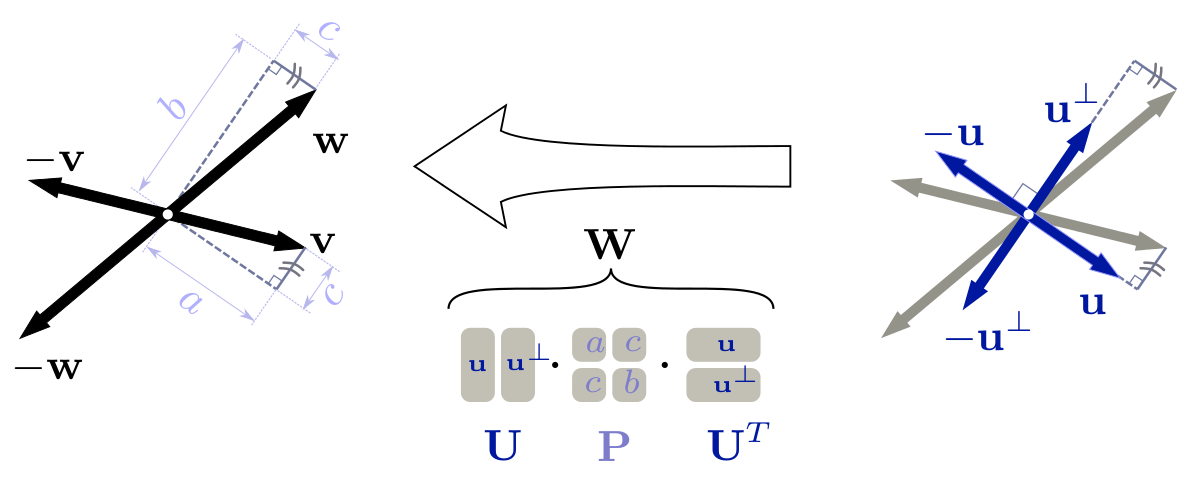
\includegraphics[width=.7\textwidth]{frame_field.png}
    \caption{Frame field示意图,图来自\cite{isotopic-appro}}
    \label{fig:frame-field}
\end{figure}
在得到一个能够充分体现原网格上的各项异性信息的标架场后,我们通过优化标架场上的一个能量将其变为尽可能各项同性的标架场,从而使得网格形变成为一个各项同性的网格。一个正交的标架$< u, u^\bot , −u, −u^\bot >, |u| = 1$,称为cross。我们知道对于任意的一个标架场$f_p = <v, w, −v, −w >$,我们都可以在切平面$T_p S$上找到一个唯一的cross $x =<u, u^\bot , −u, −u^\bot >$和同样在该切平面上的唯一的一个线性并正定(SPD)的映射W,通过它们组合表示$f_p$,$f_p = Wx = <Wu, Wu^\bot, -Wu, -Wu^\bot>$。从而,在S上的一个标架场可以唯一的分解为一个cross场X和一个SPD张量(tensor)场W。在我们离散的三角网格上,我们将标架场离散地定义到每一个三角面片上,即每一个三角面片上均有一个标架。从而在每一个三角面片 t 上,我们都可以计算出一个 corss X t 和一个由X t 到f t 映射变换W t 。很容易发现我们在三角面片t上的一个理想的形变是W t−1 ,这样就可以使得形变后的三角面片的 local size 在各个方向上都相等。然而现实中很难将所有的三角面片全部变形到最理想的状态,参照[XXXX]中的方法,并根据我们的需求——需要使得主曲率方向上的 local size尽可能一致,做一个修改,我们通过优化如下能量来计算每个三角面片 t 上的形变雅克比$J_t$:
